\documentclass{article}

\title{Lab 6}
\author{George Onwubuya}
\usepackage{fancyvrb}
\usepackage{minted}
\usepackage{graphicx}

\begin{document}
\maketitle

\section{Histogram}
\subsection{Output}
\VerbatimInput{./histogram.sh.o742644}

\subsection{Performance Analysis (4096 Bins)} 
 \setlength{\parindent}{1cm}
 \begin{tabular}{ |p{2.5cm}||p{2cm}|p{2cm}|p{2cm}|p{2cm}|p{2cm}|  }
 \hline
 \multicolumn{6}{|c|}{Execution Time (seconds) for Each Process } \\
 \hline
Elements(m) & Setting Up & DeviceVar & HostToDevice & Kernel & DeviceToHost\\
 \hline
 100000 & 0.002114 & 0.000280 & 0.000272 & 0.000452 & 0.000039\\
 \hline
 200000 & 0.003954 & 0.000304 & 0.000484 & 0.000466 & 0.000040\\
 \hline
 400000 & 0.008680 & 0.000328 & 0.000805 & 0.000458 & 0.000039\\
 \hline
 800000 & 0.017020 & 0.000258 & 0.001406 & 0.000510 & 0.000043\\
 \hline
 1000000 & 0.022502 & 0.000264 & 0.001899 & 0.000525 & 0.000041\\
 \hline
 1600000 & 0.033799 & 0.000311 & 0.002794 & 0.000543 & 0.000040\\
 \hline
 \end{tabular}
 
\subsubsection{Comments} 
 When setting up the shell script file, the number of elements were varied but I chose to use the same number of bins, 4096. The time taken to allocate device variables and copy from device to host are approximately the same. This is because the same number of variables are allocated regardless of the size of the array of input elements. The times taken to set up the problem, copy from host to device and launching the kernel are all directly proportional to the size of the input array.   

\section{Histogram (Optimized)}
\subsection{Output}
\VerbatimInput{./histogram.sh.o742646}

\subsection{Performance Analysis}
 \subsubsection{Array Size} 
 \setlength{\parindent}{1cm}
 \begin{tabular}{ |p{2.5cm}||p{2cm}|p{2cm}|p{2cm}|p{2cm}|p{2cm}|  }
 \hline
 \multicolumn{6}{|c|}{Execution Time (seconds) for Each Process } \\
 \hline
Elements(m) & Setting Up & DeviceVar & HostToDevice & Kernel & DeviceToHost\\
 \hline
 100000 & 0.002145 & 0.000262 & 0.000236 & 0.000498 & 0.000036\\
 \hline
 200000 & 0.004105 & 0.000303 & 0.000387 & 0.000504 & 0.000042\\
 \hline
 400000 & 0.008779 & 0.000259 & 0.000713 & 0.000528 & 0.000041\\
 \hline
 800000 & 0.016875 & 0.000261 & 0.001438 & 0.000560 & 0.000041\\
 \hline
 1000000 & 0.021037 & 0.000290 & 0.001656 & 0.000589 & 0.000040\\
 \hline
 1600000 & 0.033860 & 0.000284 & 0.002730 & 0.000629 & 0.000040\\
 \hline
 \end{tabular}

\subsubsection{Comments} 
 The execution times relate to the same way to the initial histogram kernel that had no optimization. 

\subsection{Answers}
\subsubsection{Description of Optimization}
To optimize the histogram kernel, the kernel code was written such that a location in shared memory would only be updated once. Three new variables were introduced to the kernel code. The first two variables current index and previous index were meant to keep track of the elements from the input array. The current index and previous were compared to check if the same element was still being evaluated because of possible repetitions in data. If they were found to be the same, a third variable accumulator would store the number of times this element occurred in succession in the array . However if the elements were not the same, the value in the accumulator would be written to a location in shared memory as indicated by the previous index, the previous index would then be set to the current index and the value in the accumulator would be set to one to indicate a shift to the next element. The accumulator and the previous index variables were initialized to zero outside the while loop and the current index variable was set to the current input element under evaluation by the histogram kernel code. 
\\
\\
\begin{figure}[h]
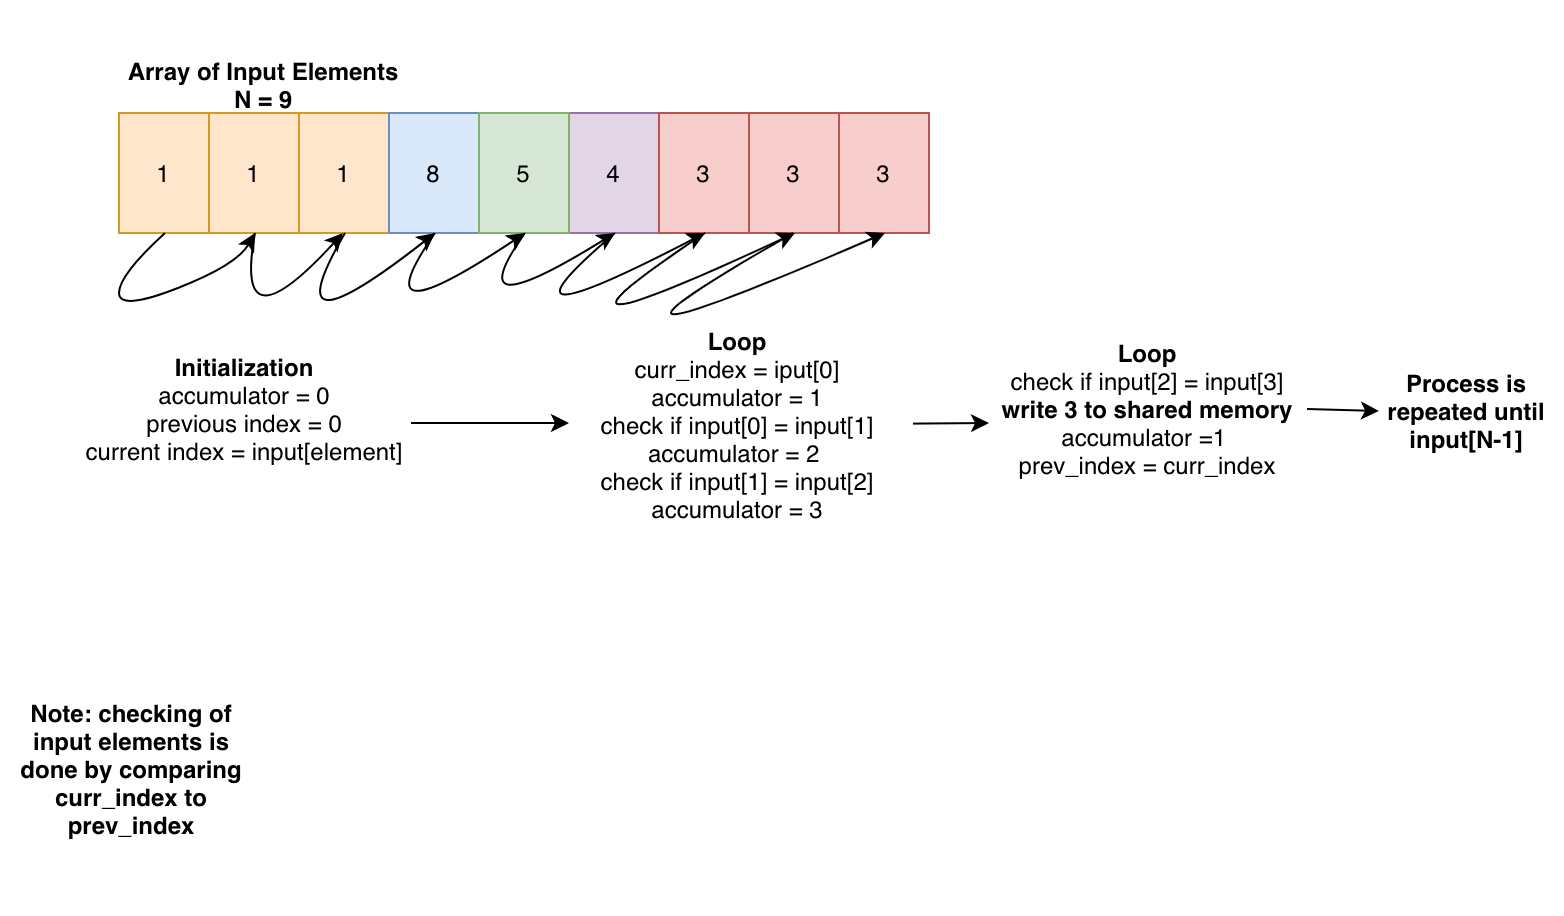
\includegraphics[width=\textwidth]{Illustration_Diagram.png}
\caption{An illustration of what the kernel code does}
\center
\end{figure}

\subsubsection{Difficulties with Optimization}
A couple of difficulties I experienced during this optimization were found in not analyzing the the second while loop structure of the code that is used to update the value in the accumulator to the shared memory location. I examined how the loop would behave at the beginning of the and during the middle part of the execution and neglected to check what happens when the loop ends. As a result my code was incomplete and was unable to simulate past the first bin. I also made the mistake of attempting to carry out the optimization without first checking if the code was properly written out. 
\subsubsection{Change in Execution Time}
\setlength{\parindent}{1cm}
 \begin{tabular}{ |p{2cm}||p{3cm}|p{3cm}| }
 \hline
 \multicolumn{3}{|c|}{Kernel Times in microseconds}\\
 \hline
Elements(m) & Non-Optimized & Optimized\\
 \hline
 100000 & 11.776 & 76.414\\
 \hline
 200000 & 18.367 & 82.398\\
 \hline
 400000 & 32.614 & 99.646\\
 \hline
 800000 & 63.039 & 129.12\\
 \hline
 1000000 & 77.356 & 144.09\\
 \hline
 1600000 & 120.38 & 190.17\\
 \hline
 \end{tabular}
\\
\\
\begin{figure}[h]
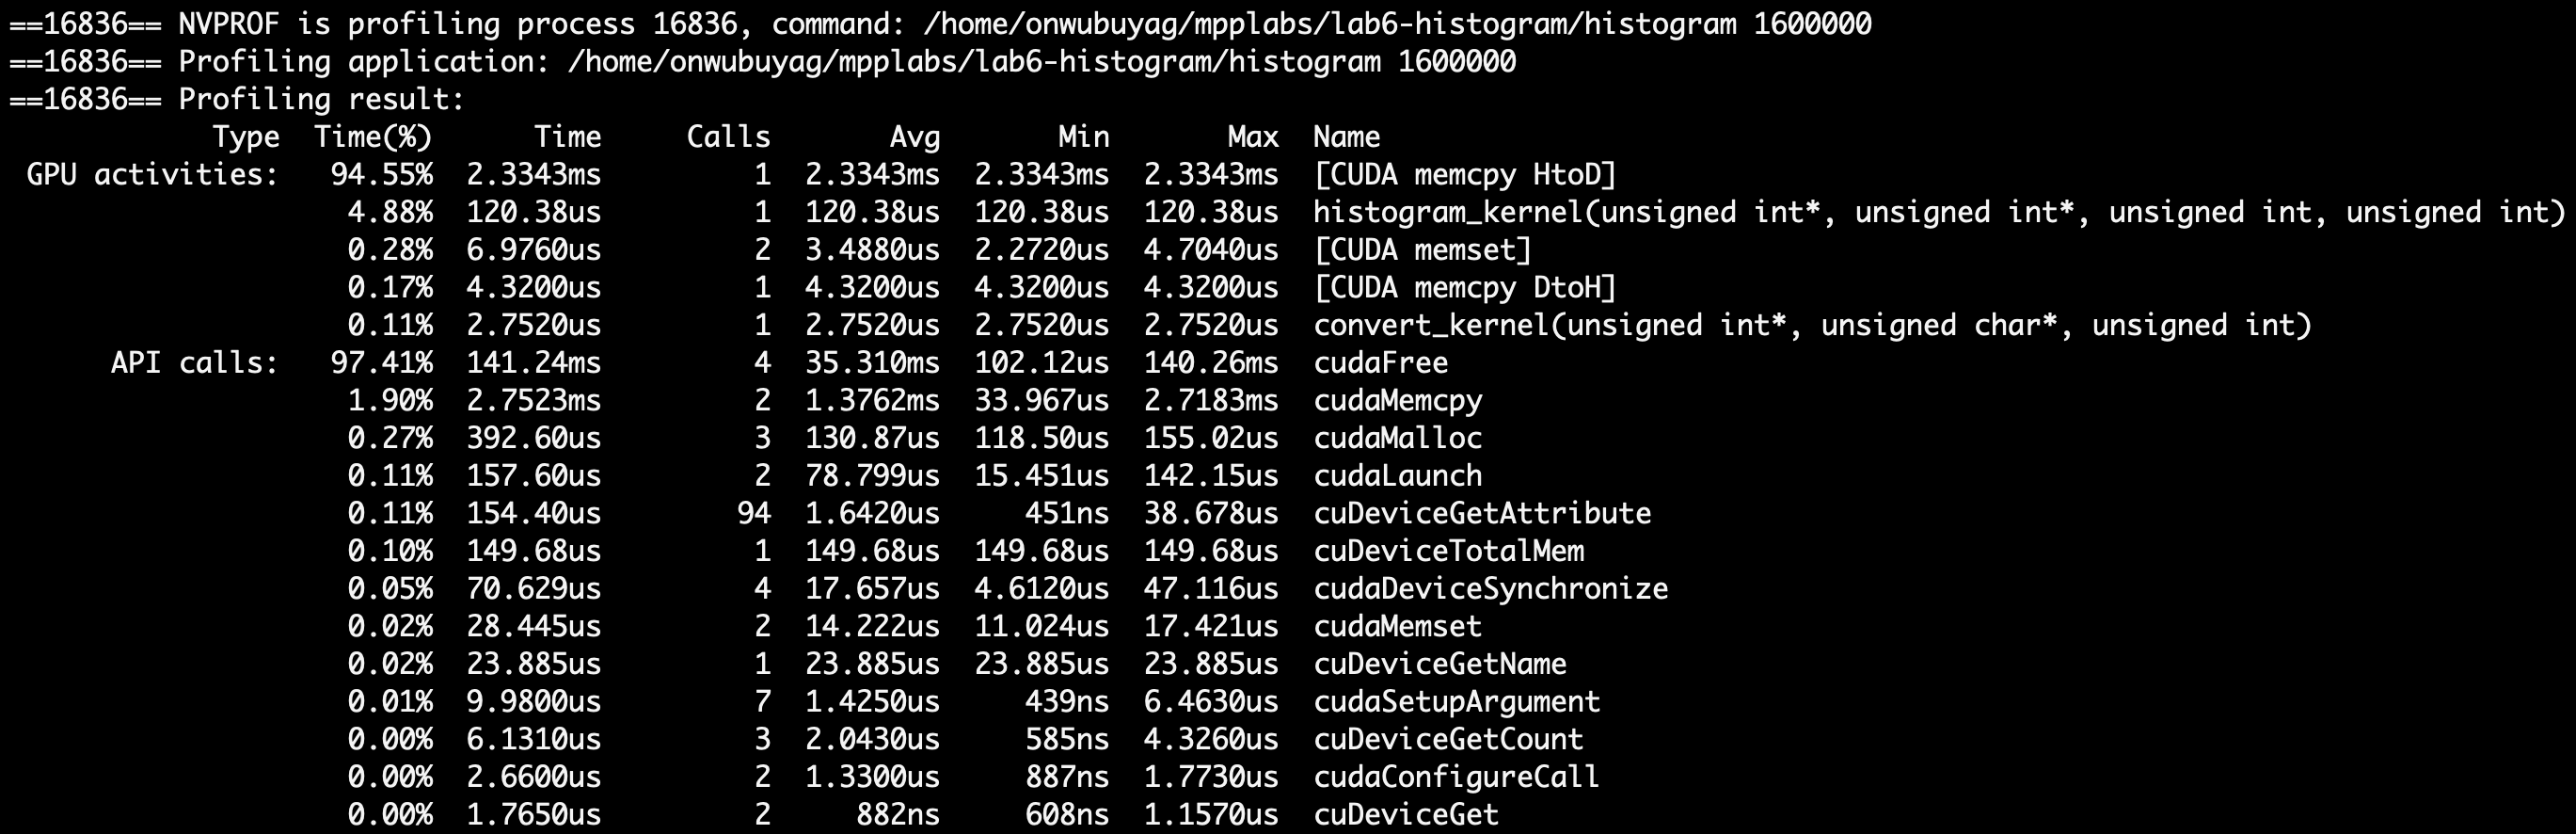
\includegraphics[width=\textwidth]{nvprof_image_1.png}
\caption{Nvidia profiler result for non-optimized histogram kernel for m = 1600000}
\center
\end{figure}
 \\
\\
\begin{figure}[h]
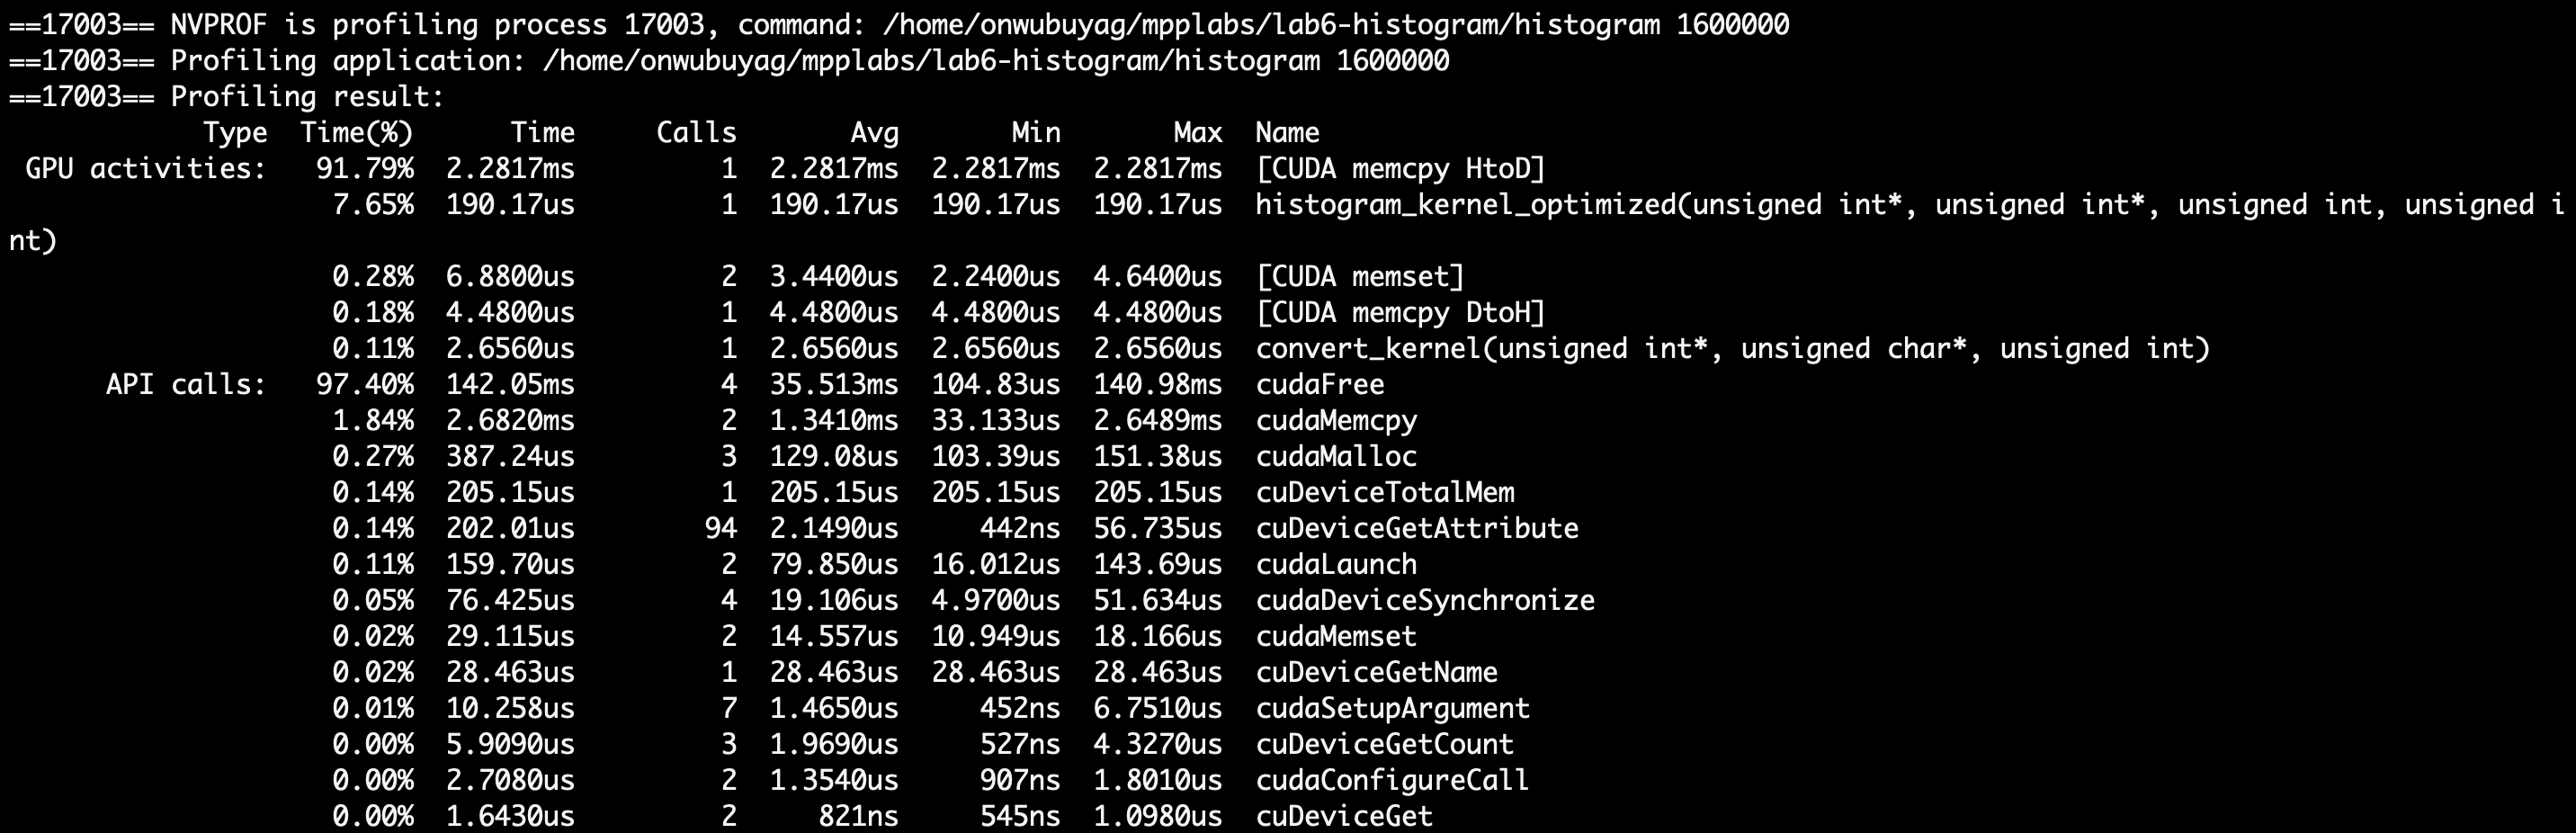
\includegraphics[width=\textwidth]{nvprof_image_2.png}
\caption{Nvidia profiler result for optimized histogram kernel for m = 1600000}
\center
\end{figure}
\\
\\
\\
\\
\\
\subsubsection{Explanation for Optimization}
The optimization increased the amount of time spent executing the kernel. I suspect that might be the result of the input array being generated with less repetition than originally anticipated. The contention rate was low and hence the addition of more variables would only serve to increase the execution time. 
\subsection{Kernel}
\inputminted[breaklines, linenos]{c}{./kernel.cu}
\end{document}
